% Week 12 report (written 2026-11-19): the first report on the comparison of the tracer with the Medis
% reference: what Medis is, how the comparison was made, and the findings. Numbers from
% CGPS_data/thesis_final/medis_compare.md (run of 2026-11-19) and the row titles of asymmetry_view.png and
% bifurcation_view.png. Steps follow research_notes/Medis comparison steps/medis_comparison_steps.tex; the
% Medis numbers follow Thesis_coronary/content/data/03_medis_reference.tex. Language after
% Thesis_coronary/content/technical/01_glm.tex.
% Numbers are \pending until medis_compare.py, curvature_view.py, bifurcation_view.py --all and asymmetry_view.py
% have been run on the server.
% Figures: weekly/week12/make_figures.py crops two rows of each figure (single participants, no ids).
% bifurcation_view.png on this Mac is from before the drawing fix of 2026-11-19 (fitted lines drawn from O);
% rerun bifurcation_view.py on the server, copy the PNG, run make_figures.py and remove the \todonote.
% 2026-11-19: each feature section opens with how the feature is computed and its method figure
% (curvature_steps_figure.png, angle_steps_figure.png, surface_cut_figure.png from
% Thesis_coronary/content/methodology/figures/, made-up shapes run through curvature_feature.py,
% bifurcation_angle.py and daughter_ratio.py; copied here by make_figures.py).
% 2026-11-19 (user: bare minimum text, the figures do the talking): every section cut to its figure and one or two
% sentences; new Figure fig:wk12-steps from centerline_steps_view.py (this folder, server only): the steps from a
% delivered Medis RCA to the compared artery for the shortest RCAs that pass the full-artery rule. Copy its PNG from
% the medis_compare rows folder to week12_figures/.
% 2026-11-19: angle and asymmetry figures from the updated bifurcation_view (1).png and asymmetry_view (1).png,
% second-worst row shown (user); make_figures.py crops them.
% 2026-11-19: numbers filled from CGPS_data/thesis_final/medis_compare.md (updated run, same day); curvature figure
% from curvature_view (1).png, second-worst row. CHECK: the diameter ICCs in medis_compare.md are on 267 / 55
% pairs while its agreement rows use 39, although the reliability table says "same pairs"; marked in the table.
% 2026-11-19 (user overruled the whole-artery-only decision): curvature is reported both over the whole artery
% and over the shared stretch (shared_curvature in medis_compare.py), from the same report.
% 2026-11-19 (user): the asymmetry is reported only as |a| (how unequal the daughters are); the signed a is removed.
% 2026-11-20: the dominance item uses the signed a on purpose (dominance shifts its sign); numbers from
% CGPS_data/thesis_final/dominance_check.md (plaque-free cohort).
% medis_compare.md has no bias or limits of agreement for |a| yet; medis_compare.py now writes them (row
% "abs(a), the model feature" in the asymmetry agreement table). Fill the dagger cells after the server run.
% 2026-11-19: Figure fig:wk12-curv-worst = worst row of CGPS_data/thesis_final/curvature_view.png (the 1,661-pair
% run before the full-artery rule), cropped by make_figures.py to curv_worst.png.
% 2026-11-19 (user): Figure fig:wk12-steps (centerline_steps_view.py, PNG never copied here) removed with its
% blue placeholders.
\documentclass[11pt,a4paper]{article}

% Week reports: author, title and supervisors from the thesis.
% ---------------------------------------------------------------
% Edit these once. Every weekly report and the thesis title page
% pick them up.
% ---------------------------------------------------------------
\newcommand{\projecttitle}{Your thesis title goes here}
\newcommand{\course}{Master Thesis}

% Supervisors, one per line. Used on the weekly title page and the
% thesis cover.
\newcommand{\supervisorlist}{%
  Rasmus R. Paulsen\\
  Kit Mills Bransby \\
  Philip Ruessell Pedersson}

\newcommand{\authorname}{Mathilde Brinch Sørensen}
\newcommand{\studentnumber}{s254124}
\newcommand{\authorline}{\authorname\ (\studentnumber)}

% Date of the current report. Override it in each weekNN.tex with
% \renewcommand{\reportdate}{January 22, 2026}
\newcommand{\reportdate}{\today}

% ---------------------------------------------------------------
% Cover page and information page (page 2). Edit these once.
% ---------------------------------------------------------------
\newcommand{\thesisperiod}{3.\ February 2026 - 3.\ August 2026}
\newcommand{\thesisects}{35 ECTS points}

% Cover image: put the file in figures/ (leave as is to skip it)
\newcommand{\coverimagefile}{coverimage.png}

% "Author" or "Authors" (also used on the cover)
\newcommand{\thesisauthorlabel}{Author}
\newcommand{\thesisauthorsuffix}{}      % set to s for several authors

% --- Cover: one line per person, separated by \\ -----------------
\newcommand{\coverauthors}{\authorname\ (\studentnumber)}
\newcommand{\coversupervisors}{%
  [Title] Rasmus R. Paulsen\\[0pt]
  [Title] Kit Mills Bransby\\[0pt]
  [Title] Philip Ruessell Pedersson}

% --- Page 2 ------------------------------------------------------
% \thesisauthor{Name (student number)}{Programme}{Institution}
\newcommand{\thesisauthor}[3]{#1\par #2\par #3\par\vspace{15.3pt}}
% \thesissupervisor{Title and name}{Affiliation}
\newcommand{\thesissupervisor}[2]{#1\par #2\par\vspace{15.3pt}}

\newcommand{\thesisauthors}{%
  \thesisauthor{\authorname\ (\studentnumber)}{M.Sc. [Your programme]}{Technical University of Denmark}}

\newcommand{\thesissupervisors}{%
  \thesissupervisor{[Title] Rasmus R. Paulsen}{[Department], Technical University of Denmark}
  \thesissupervisor{[Title] Kit Mills Bransby}{[Department / company]}
  \thesissupervisor{[Title] Philip Ruessell Pedersson}{[Department / company]}}

\newcommand{\coverphotonote}{[Describe the cover image and its sources, e.g.\ 3D rendering of \ldots].}
\newcommand{\publisher}{DTU Compute, Department of Applied Mathematics and Computer Science,\newline
Richard Petersens Plads, Building 324, 2800 Kgs.\ Lyngby, Denmark}


% Week 12 preamble (copied 2026-11-19 from outdated/thesis_retired/week10/setup/preamble.tex, paths for
% weekly/week12/). Figures resolve from week12/week12_figures/.
\usepackage[T1]{fontenc}
\usepackage[utf8]{inputenc}
\usepackage{lmodern}
\usepackage[english]{babel}
\usepackage{amsmath,amssymb,mathtools}
\usepackage{graphicx}
\usepackage{float}
\usepackage[section]{placeins}  % every figure of a section is shown before the next section starts
\usepackage{booktabs,tabularx}
\usepackage{xcolor}
\usepackage{enumitem}
\usepackage[margin=2.5cm]{geometry}
\usepackage[hidelinks]{hyperref}
\usepackage{cleveref}
\graphicspath{{./}{week12_figures/}}
\providecommand{\clarify}[1]{\textcolor{red}{\textbf{Clarification needed:} #1}}
\providecommand{\todonote}[1]{\textcolor{blue}{\textbf{To do:} #1}}
\providecommand{\pending}[1]{\textcolor{blue}{\textbf{[#1]}}}  % a number waiting for the rerun of medis_compare.py

% Week report title and progress heading (rebuilt 2026-11-09).
\newcommand{\weeklytitle}[1]{%
  \begin{center}
    {\LARGE\bfseries Weekly report #1}\\[0.5em]
    {\large \projecttitle}\\[0.5em]
    \authorline\\
    \reportdate
  \end{center}\medskip}
\newcommand{\sectionprogress}{\subsection*{Progress}}


\renewcommand{\reportdate}{19 November 2026}

\begin{document}

\weeklytitle{12}

\section*{Week 12: 16--20 November 2026}

\sectionprogress

\begin{itemize}[itemsep=2pt]
  \item \textbf{I received Kit's predictions.}
  \item \textbf{I compared the tracer with Medis.} Instead of comparing the predictions directly, I compared the
    features, since these are what goes into my model: curvature, the LM bifurcation angle and the asymmetry
    between the LAD and LCx.
  \item \textbf{ICC used:} ICC(3,1), the two-way mixed-effects, consistency, single-measurement ICC (Koo and Li
    2016, Table 3); explained above Table~\ref{tab:wk12-findings}.
  \item \textbf{Curvature} (Table~\ref{tab:wk12-findings}): the tracer agrees well with Medis (ICC 0.84 over the
    whole artery, 1,191 artery pairs; 0.95 over the stretch both lines cover).
  \item \textbf{A full Medis artery can still be a stump.} Medis centerlines often stop before the end of the
    artery, and most of the curvature disagreement comes from where the lines stop, not from the curvature where
    both run: over the stretch both lines cover, the SD of the differences falls from 0.010 to 0.006\,mm$^{-1}$
    (Figure~\ref{fig:wk12-curv}).
  \item \textbf{Angle}: the tracer agrees well with Medis (ICC 0.92, 344 participants).
  \item \textbf{Asymmetry}: Medis has lumen contours only where there is plaque, so the asymmetry could be
    compared in only 39 participants. The ICC of $|a|$, how unequal the two daughters are,
    is 0.65.
  \item \textbf{Asymmetry by dominance} (known-groups check, plaque-free cohort, 880 participants): if the tracer
    measures the daughters' size, the LCx should be wider in left-dominant hearts. It is. The asymmetry
    $a = \ln(D_\text{LCx}/D_\text{LAD})$ rises from right ($-0.10$, 730) over co-dominant (0.005, 74) to left
    dominance (0.08, 76); left minus right is 0.18 (95\% CI 0.14 to 0.22, $p < 0.001$). The difference comes from
    the LCx alone ($+0.59$\,mm, LAD $+0.04$\,mm), as anatomy predicts. Fewer left-dominant hearts have an asymmetry
    (72\% against 83\% right).
\end{itemize}

\subsection*{Questions}

\begin{itemize}[itemsep=2pt]
  \item Should the asymmetry stay a main feature of the bifurcation model, become a secondary analysis, or be
    dropped? Against it: the evidence rests mainly on one computational study (Garcha and Grande Gutiérrez 2025),
    which found low wall shear stress in the smaller of the two daughters, and its ICC against Medis (0.65) is lower
    than for curvature and the angle. For it: the dominance check shows the expected difference, with the LCx wider
    in left-dominant hearts and the LAD unchanged, so the tracer measures the size of the daughters. The asymmetry
    also varies more within the dominance groups than between them, so dominance alone cannot replace it.
  \item Can I show scatter plots with one dot per participant (no ids) in the thesis and the weekly reports, for
    example the asymmetry by dominance group and the Bland--Altman plots? 
\end{itemize}

\newpage

\section*{The Medis Reference}

Medis centerlines exist for 600 participants and lumen contours only for segments with plaque, so the comparison
lies outside the plaque-free cohort. The same code runs on both trees, and nothing from Medis changes a tracer
value. Agreement is given as bias, limits of agreement and ICC (tracer minus Medis).

\section*{Curvature}

\begin{figure}[h]
  \centering
  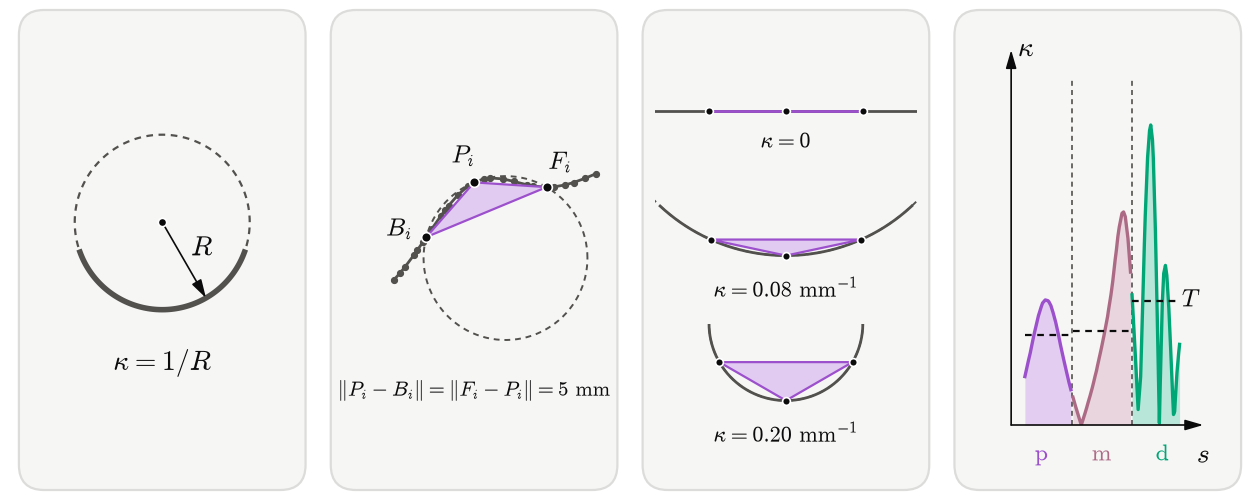
\includegraphics[width=\textwidth]{curvature_steps_figure.png}
  \caption{How curvature is computed (made-up artery, thesis code): $1/R$ of the circle through each point and
  the points 5\,mm away, the profile along the artery and its average $T$ per segment.}
  \label{fig:wk12-curv-method}
\end{figure}

Curvature is averaged over each tree's whole artery, from its own start to its own end, and compared only where
the Medis artery is full: along its path it starts in its proximal segment, ends in its distal segment and holds
all three, and is at least as long as the shortest tracer artery of its kind (LAD 18.7, LCx 12.1, RCA 14\,mm).
This keeps 475 LADs, 478 LCxs and 455 RCAs; most of the others do not end in the distal segment. Before the
rule, the largest differences came from short Medis fragments (Figure~\ref{fig:wk12-curv-worst}).

\begin{figure}[h]
  \centering
  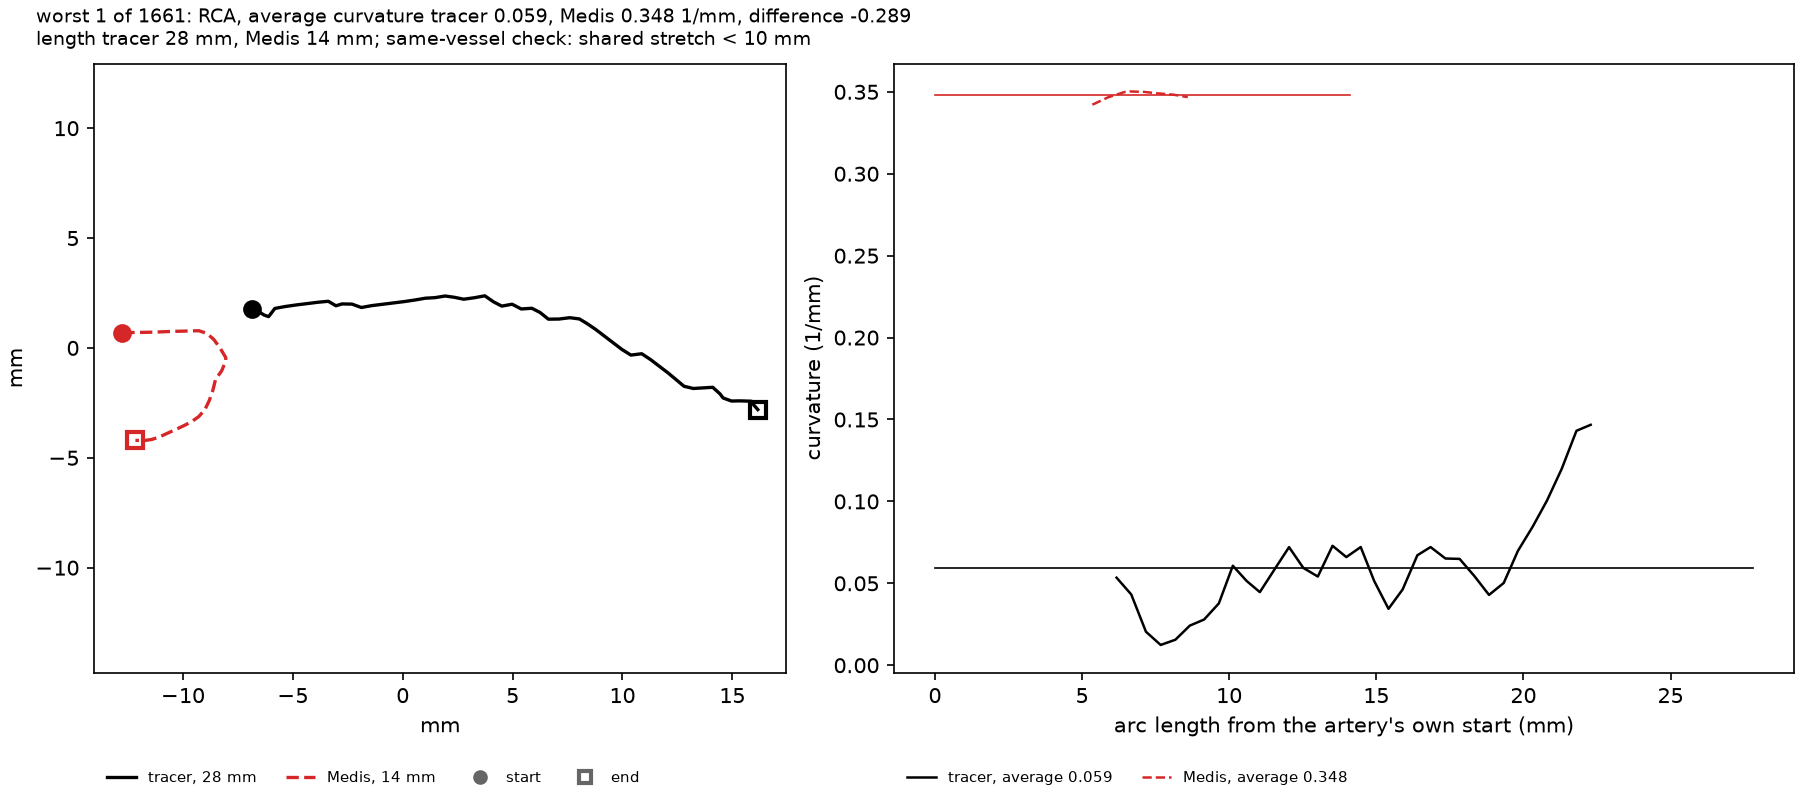
\includegraphics[width=0.9\textwidth]{curv_worst.png}
  \caption{Largest difference of 1,661 pairs, from the run before the full-artery rule. The Medis RCA is a
  14\,mm fragment that bends back on itself beside the tracer RCA. A curvature value needs a point 5\,mm on each
  side, so the Medis average rests on about 3\,mm of this bend: 0.35\,mm$^{-1}$ against 0.06\,mm$^{-1}$ for
  the tracer. The two lines share less than 10\,mm, so the pair fails the same-vessel check, and the full-artery
  rule now excludes such fragments.}
  \label{fig:wk12-curv-worst}
\end{figure}

Even so, a
full Medis artery can stop well before the tracer's (Figure~\ref{fig:wk12-curv}, top).

Curvature: 1,191 pairs, bias 0.005\,mm$^{-1}$ (tracer higher), limits $-0.015$ to 0.025\,mm$^{-1}$, ICC 0.84
(LAD 0.87, LCx 0.78, RCA 0.86). The tracer had a value for 95\% to 99\% of the full Medis arteries.
Averaged over the shared stretch only (the stretch both lines cover, less 5\,mm at each end, at least 10\,mm):
1,184 pairs, bias 0.005\,mm$^{-1}$, limits $-0.006$ to 0.016\,mm$^{-1}$, ICC 0.95 (LAD 0.94, LCx 0.96, RCA 0.95).
On the same pairs the SD of the differences falls from 0.010 to 0.006\,mm$^{-1}$, so most of the whole-artery
disagreement comes from where the lines stop.

\begin{figure}[h]
  \centering
  \IfFileExists{week12_figures/curv_bad.png}{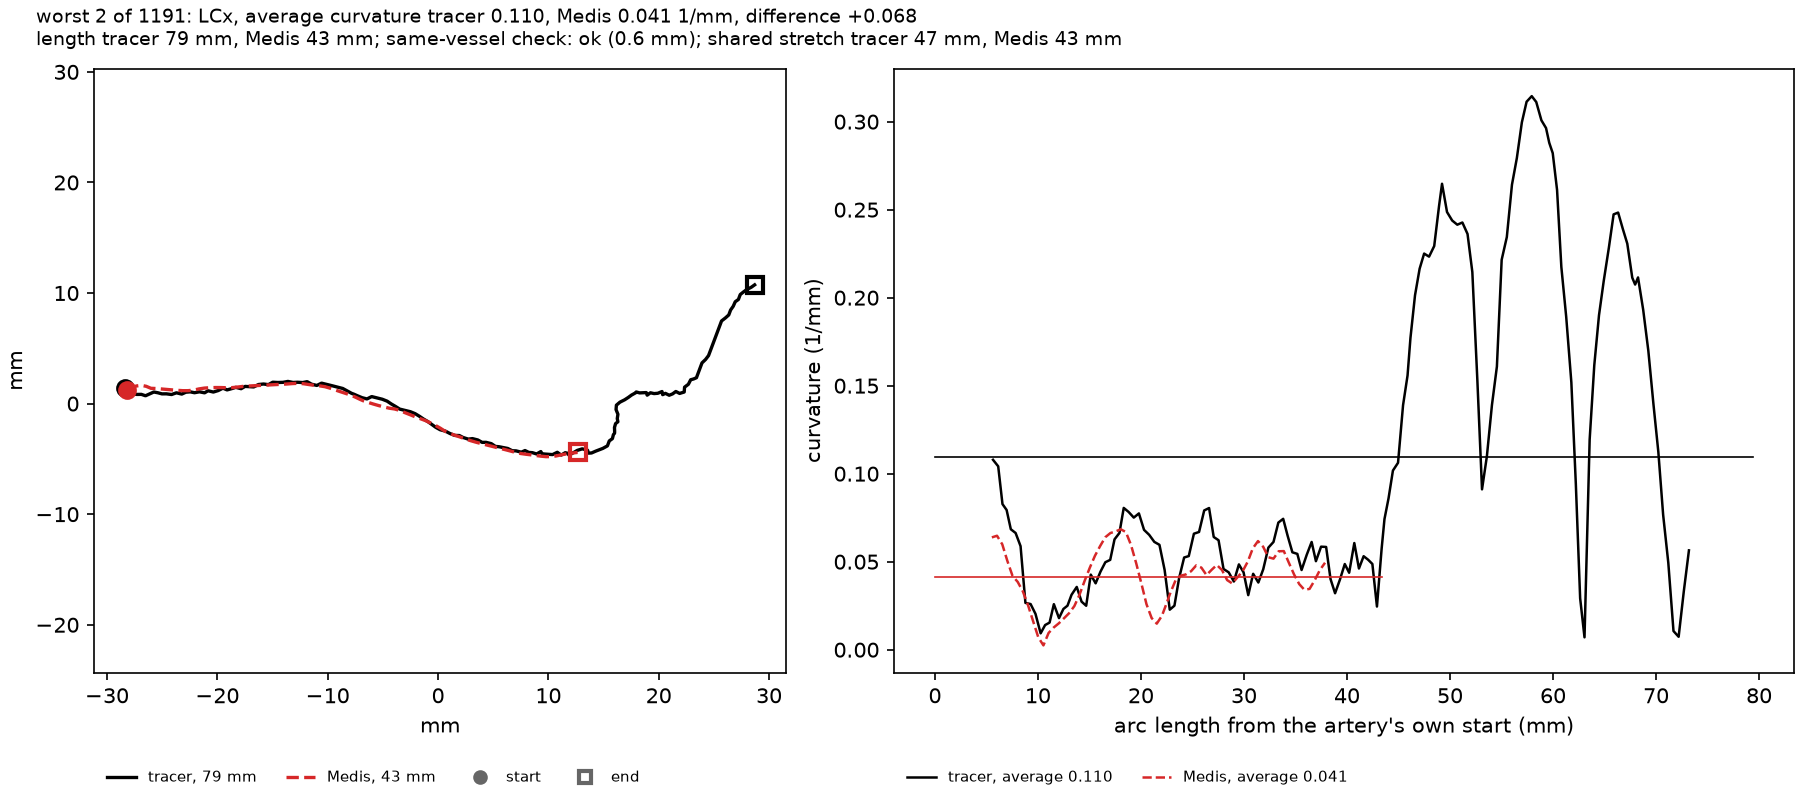
\includegraphics[width=0.9\textwidth]{curv_bad.png}\\[2pt]
    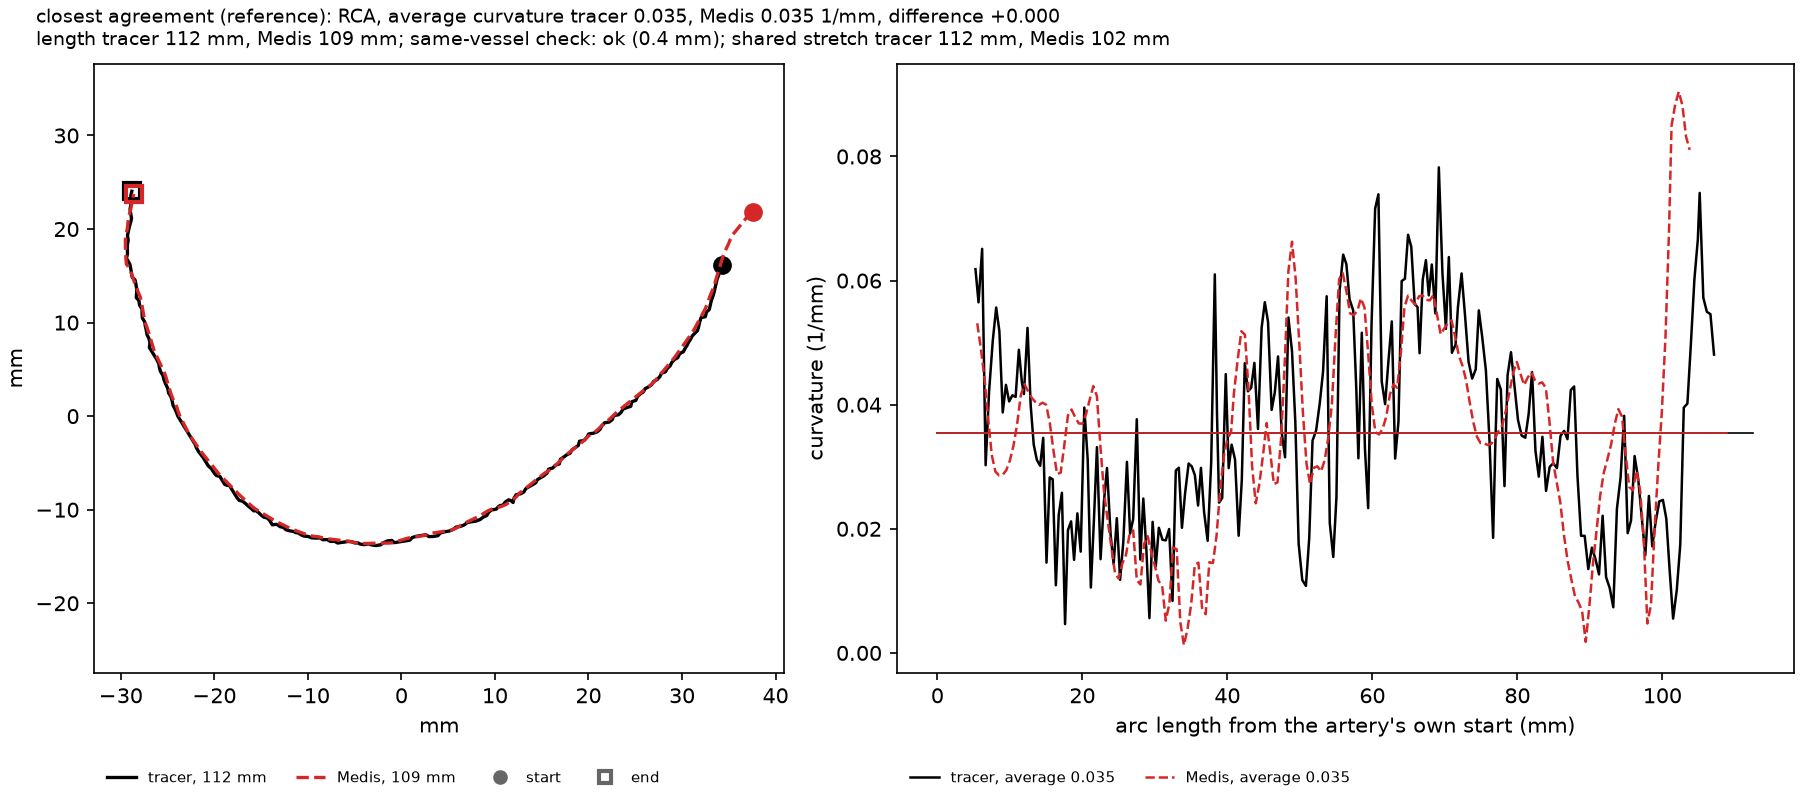
\includegraphics[width=0.9\textwidth]{curv_good.png}}{\pending{figure: curvature\_view.py}}
  \caption{Second-largest difference of 1,191 pairs (top) and closest agreement (bottom): the artery of both
  trees (tracer solid, Medis dashed; start circle, end square) and the curvature along each with its average.
  At the top, a full Medis LCx of 43\,mm follows the tracer closely and has the same curvature where both run,
  but the tracer continues to 79\,mm through tight bends, which raise its average from about 0.04 to
  0.11\,mm$^{-1}$.}
  \label{fig:wk12-curv}
\end{figure}

\newpage
\section*{Bifurcation Angle}

\begin{figure}[h]
  \centering
  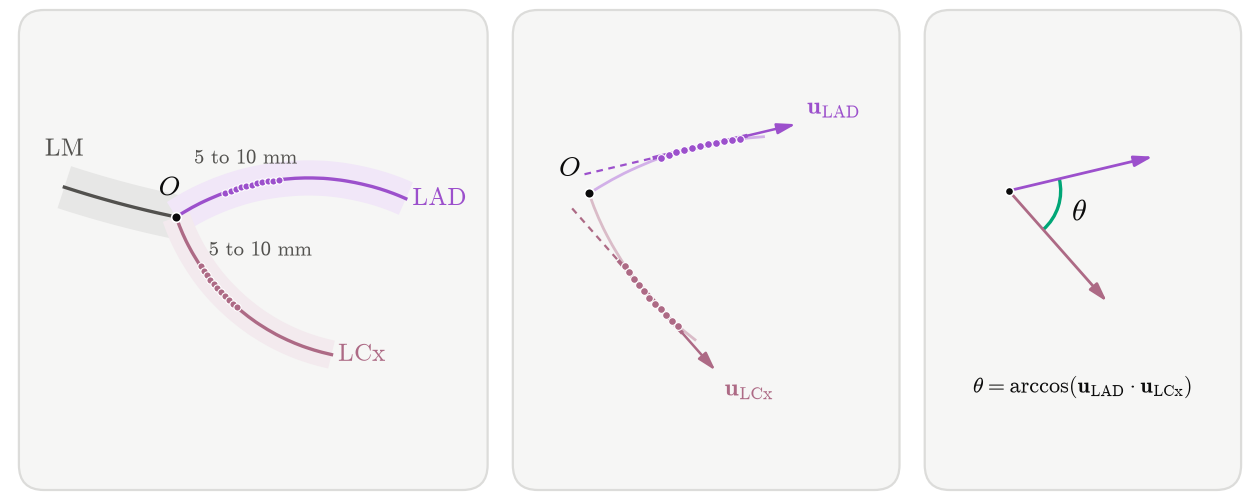
\includegraphics[width=\textwidth]{angle_steps_figure.png}
  \caption{How the angle is computed (made-up bifurcation). O is the point where the left main divides into the
  LAD and the LCx. Points 5 to 10\,mm from O, a line
  fitted through each set, and the angle $\theta$ between their directions.}
  \label{fig:wk12-angle-method}
\end{figure}

Angle: 344 participants, bias 1.1 degrees, limits $-18.7$ to 20.8 degrees, ICC 0.92
(Figure~\ref{fig:wk12-angle}). The tracer had an angle in 504 of the 543 participants with a Medis angle (93\%);
most of the others have no LM label. 

\begin{figure}[h]
  \centering
  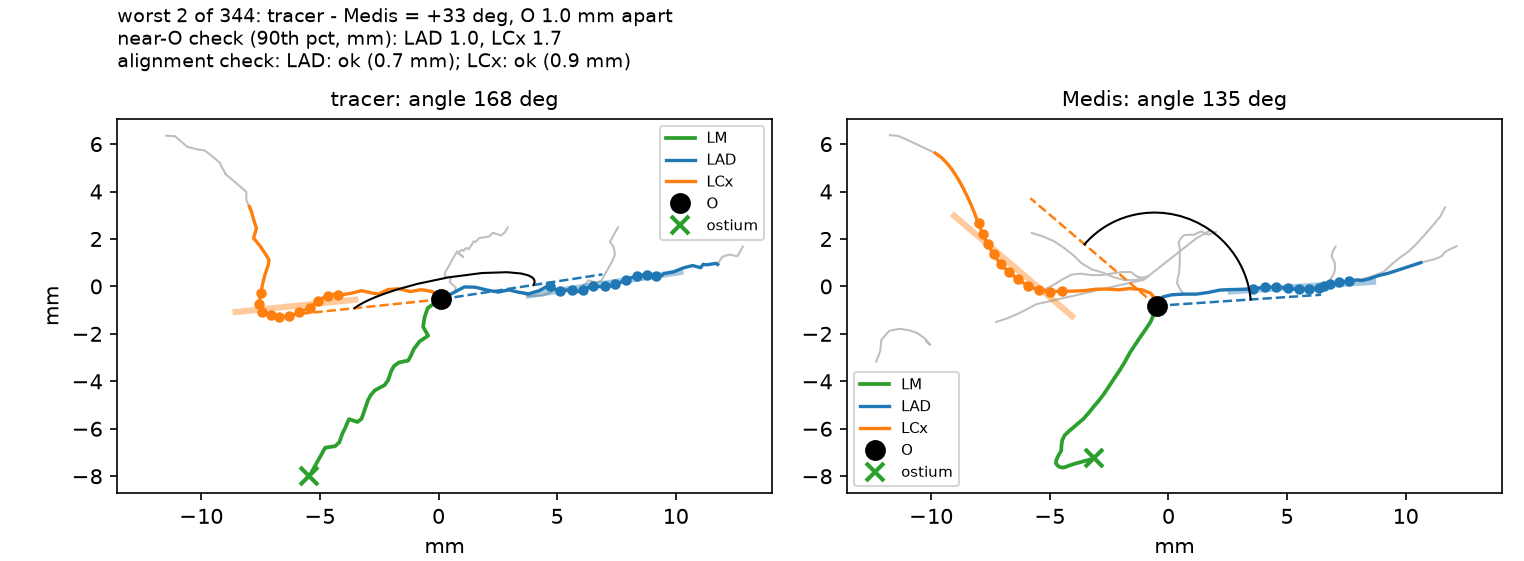
\includegraphics[width=0.62\textwidth]{angle_bad.png}\\[2pt]
  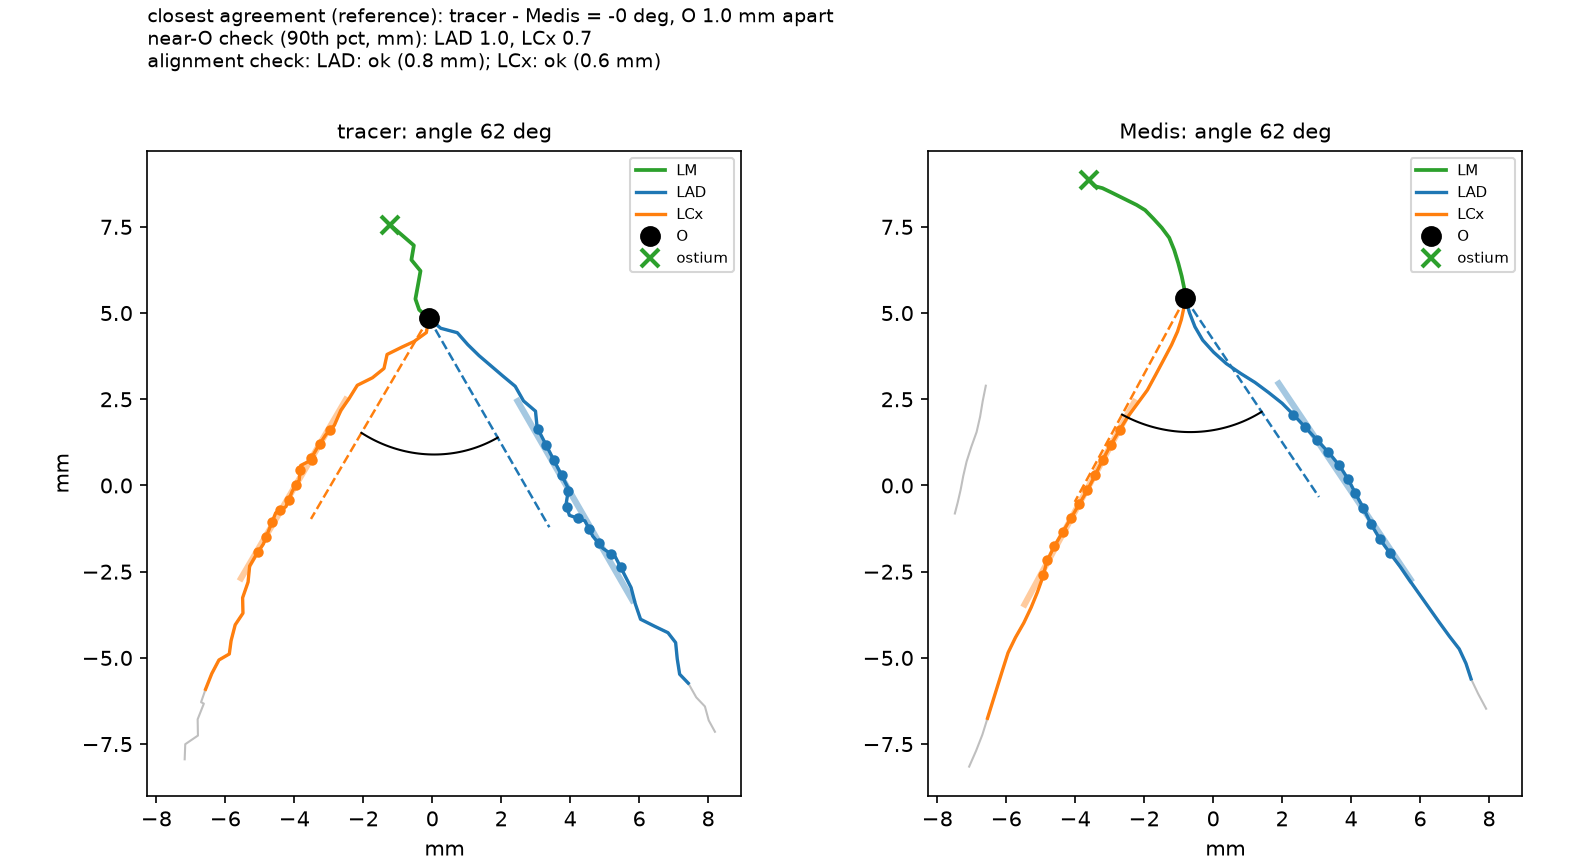
\includegraphics[width=0.62\textwidth]{angle_good.png}
  \caption{Second-largest difference (top) and closest agreement (bottom) of 344 compared participants: LM, LAD
  and LCx, the points 5 to 10\,mm from O and the fitted lines.}
  \label{fig:wk12-angle}
\end{figure}
\newpage
\section*{Daughter Asymmetry}

\begin{figure}[h]
  \centering
  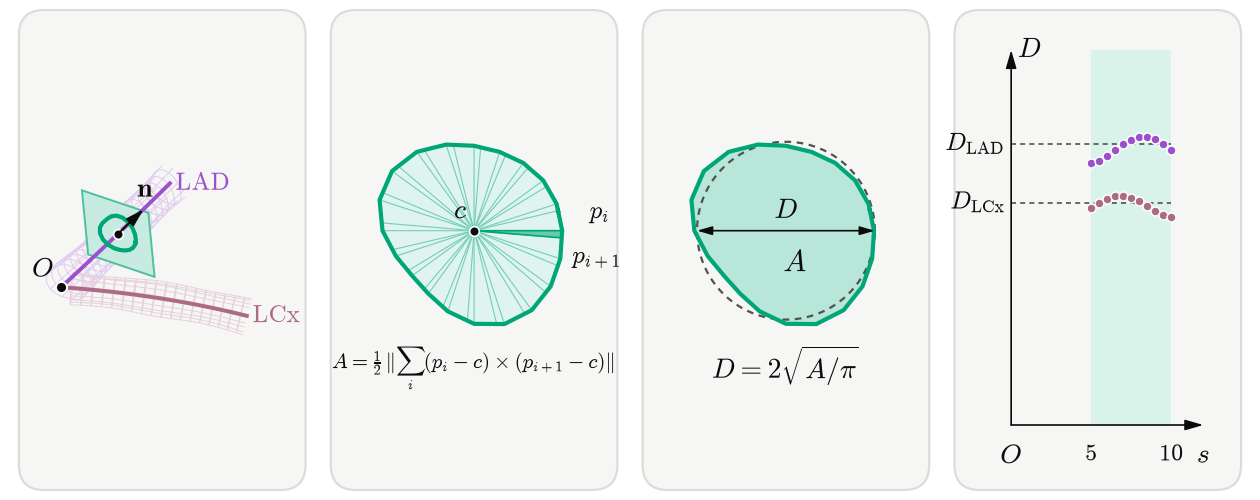
\includegraphics[width=\textwidth]{surface_cut_figure.png}
  \caption{How the diameters are computed (made-up bifurcation, thesis code): the lumen mesh cut at right angles
  to the centerline, the area of the cut, the circle with the same area, and the median over the 11 cuts 5 to
  10\,mm from O. A daughter has a diameter only when all 11 cuts work; the asymmetry is $|a| = |\ln(D_{\mathrm{LCx}}/D_{\mathrm{LAD}})|$.}
  \label{fig:wk12-asym-method}
\end{figure}

Asymmetry $|a|$: 39 participants, SD of differences 0.096 against 0.116 between people, ICC 0.65
(Figure~\ref{fig:wk12-asym}). Medis covers 5 to 10\,mm from O only where it was contoured, so the asymmetry
could be compared in only 39 participants. The tracer reads $|a|$ slightly higher
(bias 0.02, limits $-0.17$ to 0.21), and both tracer diameters are smaller than Medis (LAD $-0.19$\,mm,
LCx $-0.16$\,mm).

\begin{figure}[h]
  \centering
  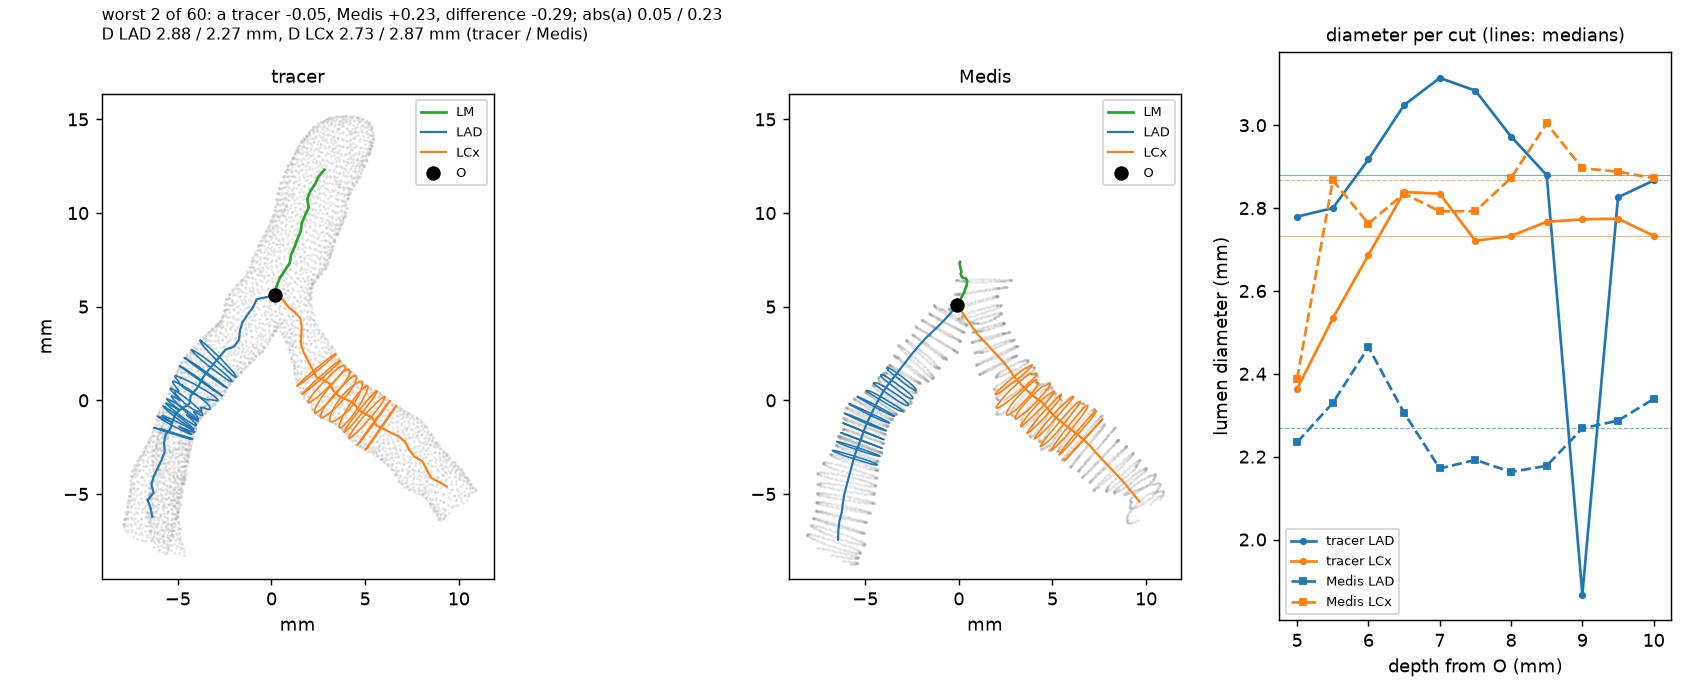
\includegraphics[width=0.9\textwidth]{asym_bad.png}\\[2pt]
  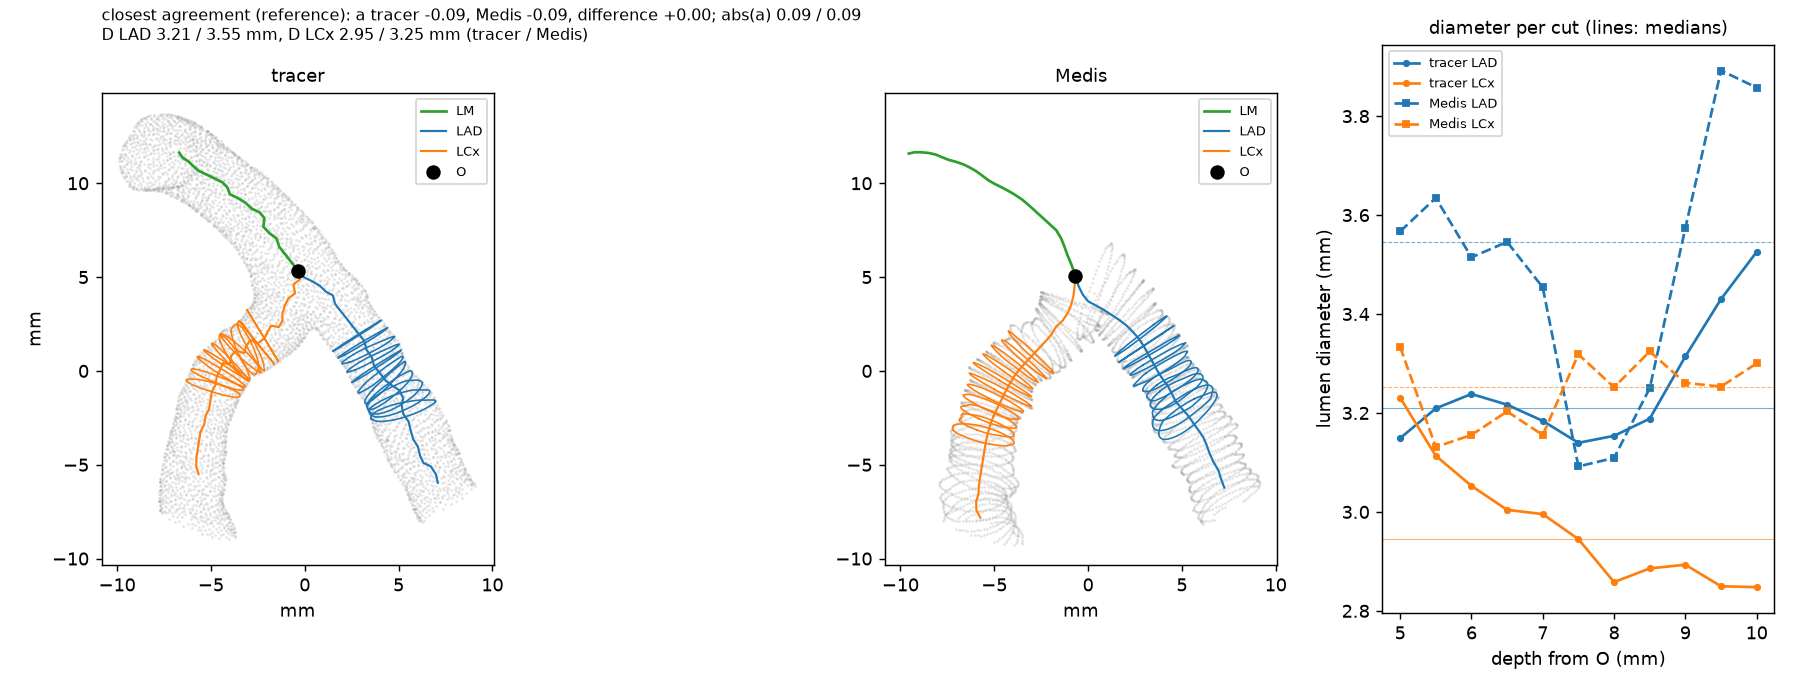
\includegraphics[width=0.9\textwidth]{asym_good.png}
  \caption{Second-largest difference (top) and closest agreement (bottom): the lumen
  with the cut at each depth (LAD blue,
  LCx orange) and the diameter of each cut (tracer solid, Medis dashed, thin lines the medians).}
  \label{fig:wk12-asym}
\end{figure}


\section*{Agreement}

Each pair is one artery measured twice, so any difference within a pair is measurement disagreement. The
intraclass correlation coefficient (ICC) compares this disagreement with how much the feature varies from one
person to another: it is the share of the total variance that lies between people. It is 1 when the tracer and
Medis give the same value for every pair, 0.5 when the disagreement within pairs is as large as the differences
between people, and near 0 when it swamps them. I used the two-way mixed-effects, consistency, single-measurement
ICC, ICC(3,1) (Koo and Li 2016, Table 3), computed per feature on the same-vessel pairs from a two-way ANOVA with
the pairs as rows and the tracer and Medis as the two columns. This form ignores a constant bias, since a constant
shift does not change a hazard ratio per SD; the bias is reported separately. The 95\% CI comes from 2,000
bootstrap samples of participants. Medis is not ground truth, so the ICC measures agreement, not accuracy. It also
grows with the spread between people, so a value from the plaque participants need not hold in the plaque-free
cohort.

\begin{table}[h]
  \centering
  \small
  \setlength{\tabcolsep}{3pt}
  \begin{tabular}{@{}lrrrrrrr@{}}
    \toprule
    Feature & Pairs & \begin{tabular}[b]{@{}c@{}}Mean\\(tracer)\end{tabular} & Bias & \begin{tabular}[b]{@{}c@{}}Limits of\\agreement\end{tabular} & \begin{tabular}[b]{@{}c@{}}SD of\\differences\end{tabular} & \begin{tabular}[b]{@{}c@{}}SD between\\people\end{tabular} & ICC \\
    \midrule
    Curvature, whole (1/mm) & 1,191 & 0.062 & 0.005 & $-0.015$ to 0.025 & 0.010 & 0.019 & 0.84 \\
    \quad in degrees/mm & & 3.53 & 0.29 & $-0.87$ to 1.44 & 0.59 & 1.10 & \\
    Curvature, shared (1/mm) & 1,184 & 0.061 & 0.005 & $-0.006$ to 0.016 & 0.006 & 0.019 & 0.95 \\
    \quad in degrees/mm & & 3.47 & 0.30 & $-0.34$ to 0.94 & 0.33 & 1.09 & \\
    LAD--LCx angle (degrees) & 344 & 75.6 & 1.1 & $-18.7$ to 20.8 & 10.1 & 26.9 & 0.92 \\
    Asymmetry $|a|$ & 39 & 0.16 & 0.02 & $-0.17$ to 0.21 & 0.096 & 0.116 & 0.65 \\
    LAD diameter (mm) & 39 & 3.28$^{*}$ & $-0.19$ & $-0.82$ to 0.45 & 0.325 & 0.57$^{*}$ & 0.89$^{*}$ \\
    LCx diameter (mm) & 39 & 3.18$^{*}$ & $-0.16$ & $-0.45$ to 0.14 & 0.150 & 0.60$^{*}$ & 0.95$^{*}$ \\
    \bottomrule
  \end{tabular}
  \caption{Agreement of the tracer with Medis (tracer minus Medis), same-vessel pairs. Mean: the tracer's mean over the pairs; the Medis mean is about the tracer mean minus the bias. Limits of agreement: bias $\pm$ 1.96 SD of differences, the range that holds the difference between the tracer and Medis for about 95\% of pairs. SD between people: the SD of the tracer feature over the pairs, how much the feature varies from person to person; the error matters when the SD of differences is large next to it. ICC(3,1), consistency. Curvature over the whole artery and over the stretch both lines cover. Curvature in degrees/mm is the turning of the centerline per mm, 1/mm $\times\ 180/\pi$.
  $^{*}$The diameter means, SDs between people and ICCs are on 267 (LAD) and 55 (LCx) pairs, not the 39 of the agreement columns.}
  \label{tab:wk12-findings}
\end{table}

Curvature and the angle agree well; the tracer reads curvature slightly higher (0.062 against 0.057\,mm$^{-1}$, about 9\%), which does
not change a hazard ratio per SD. Over the shared stretch curvature agrees closely (ICC 0.95); the whole-artery value is lower (0.84)
because the lines stop at different places. The weak point is $|a|$: few pairs, a moderate ICC, and tracer diameters about 0.2\,mm narrower
than Medis. All participants in the comparison have plaque, so the agreement in the plaque-free cohort may
differ.

\end{document}
